\section{Misura di \textbf{r}}

Dopo aver misurato $B$ si inserisce il bulbo nell'alloggiamento posto tra le bobine.
Si alimenta il filamento interno con una tensione sufficiente alla produzione di elettroni per effetto termoionico, si procede quindi all'alimentazione delle bobine di Helmholtz (tra \SI{6}{\volt} e \SI{9}{\volt}) e del cannone elettronico (tra \SI{200}{\volt} e \SI{300}{\volt}).
	
%Per i valori di $V_{coil}$ e $V_{acc}$ appena fissati si è  osservata la variazione del pennellino elettronico al variare di 	$V_{heat}$.
%Per valori di $V_{heat}<$\SI{3}{\volt}
%non si osserva emissione di \e; ciò suggerisce la presenza di un valore di soglia
%$\sim 3 V$. Per valori $V_{heat}>$\SI{3}{\volt} ma ad esso prossimo
%si osserva che il fascio sia meno definito rispetto alle tensioni superiori;
%qesto effetto rislta compatibile col fatto che il filamento si trovi ,o termalizzi, a temperatre più basse qindi emetta %meno \e;

Si posiziona la reflex con l'asse dell'obiettivo perpendicolare al piano in cui si muovono gli elettroni, centrato rispetto al centro del bulbo.
Si procede quindi ad acquisire foto dell'apparato al variare di $B$ (controllato variando la tensione di alimentazione delle bobine e misurando $I$) e $V$ nei range sopra descritti.

In \figurename{ \ref{f:acquisizione}} si riportano alcune delle foto acquisite a titolo di esempio.
		
		\begin{figure}[H]
		\centering
		\subfloat{
			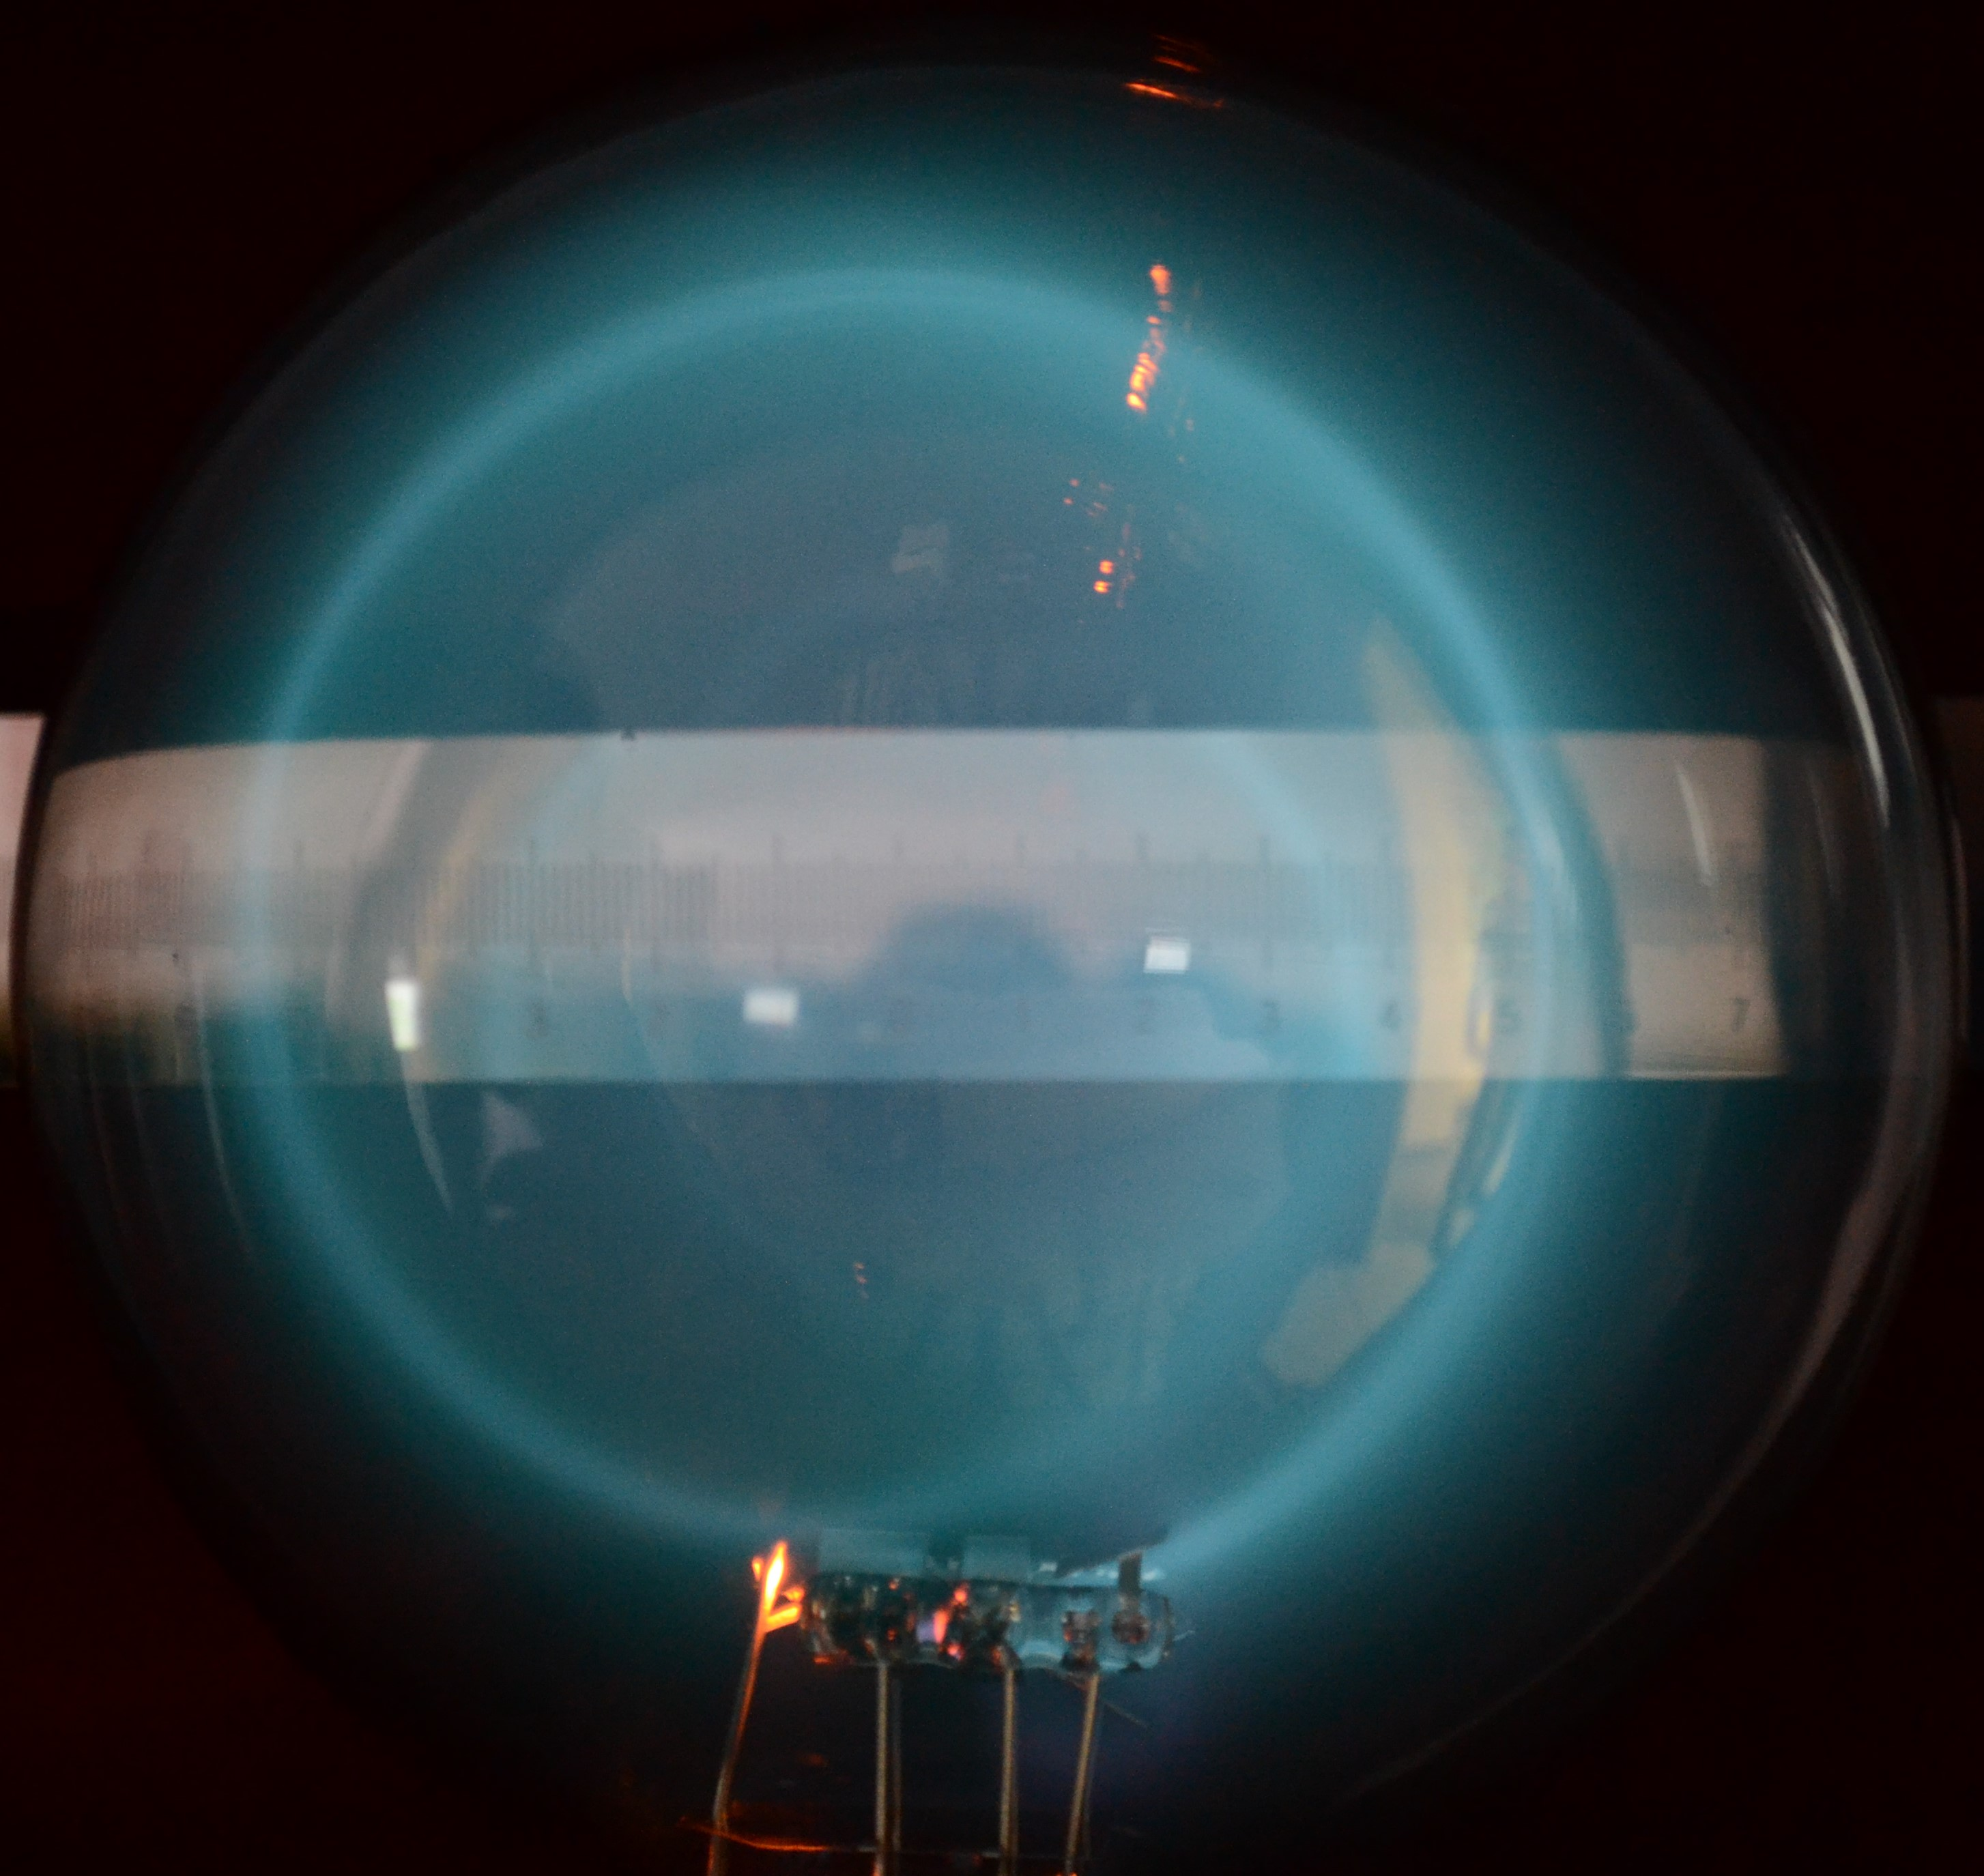
\includegraphics[scale=0.30]{(11).JPG}
			\label{stocazzo}}
		\subfloat{
			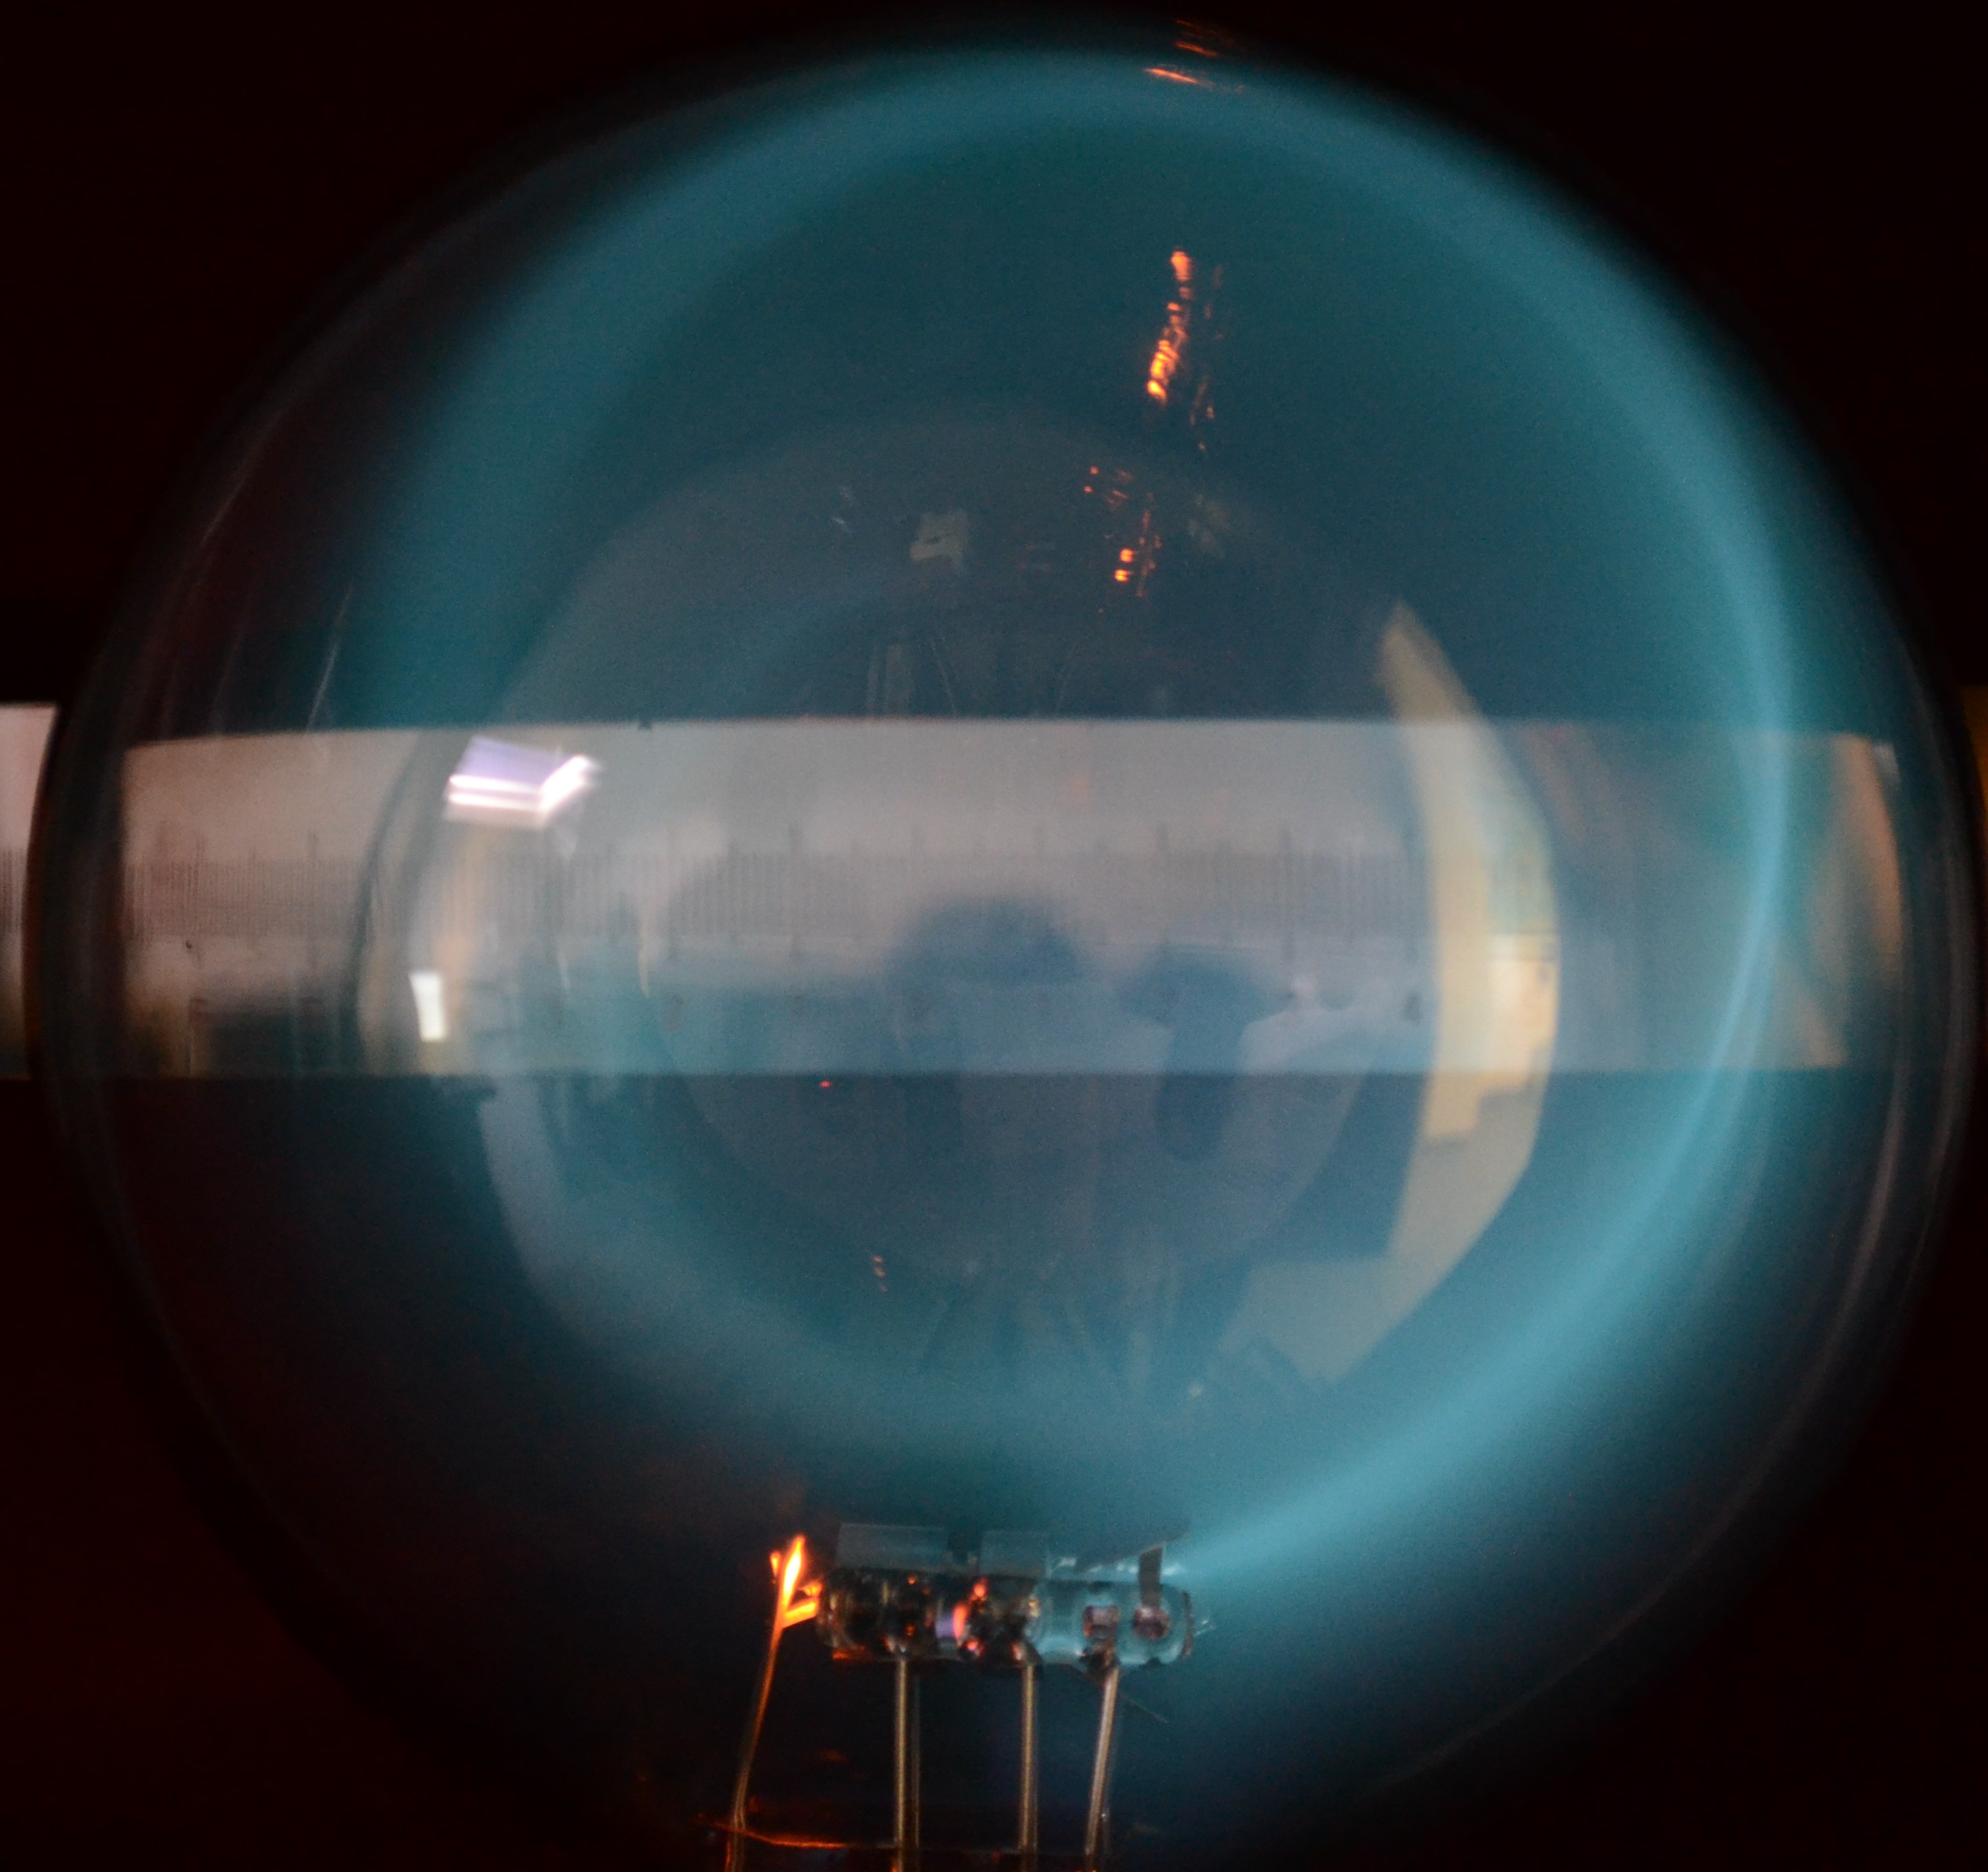
\includegraphics[scale=0.303]{(1).JPG}
			\label{coda}}\\
		\subfloat{
			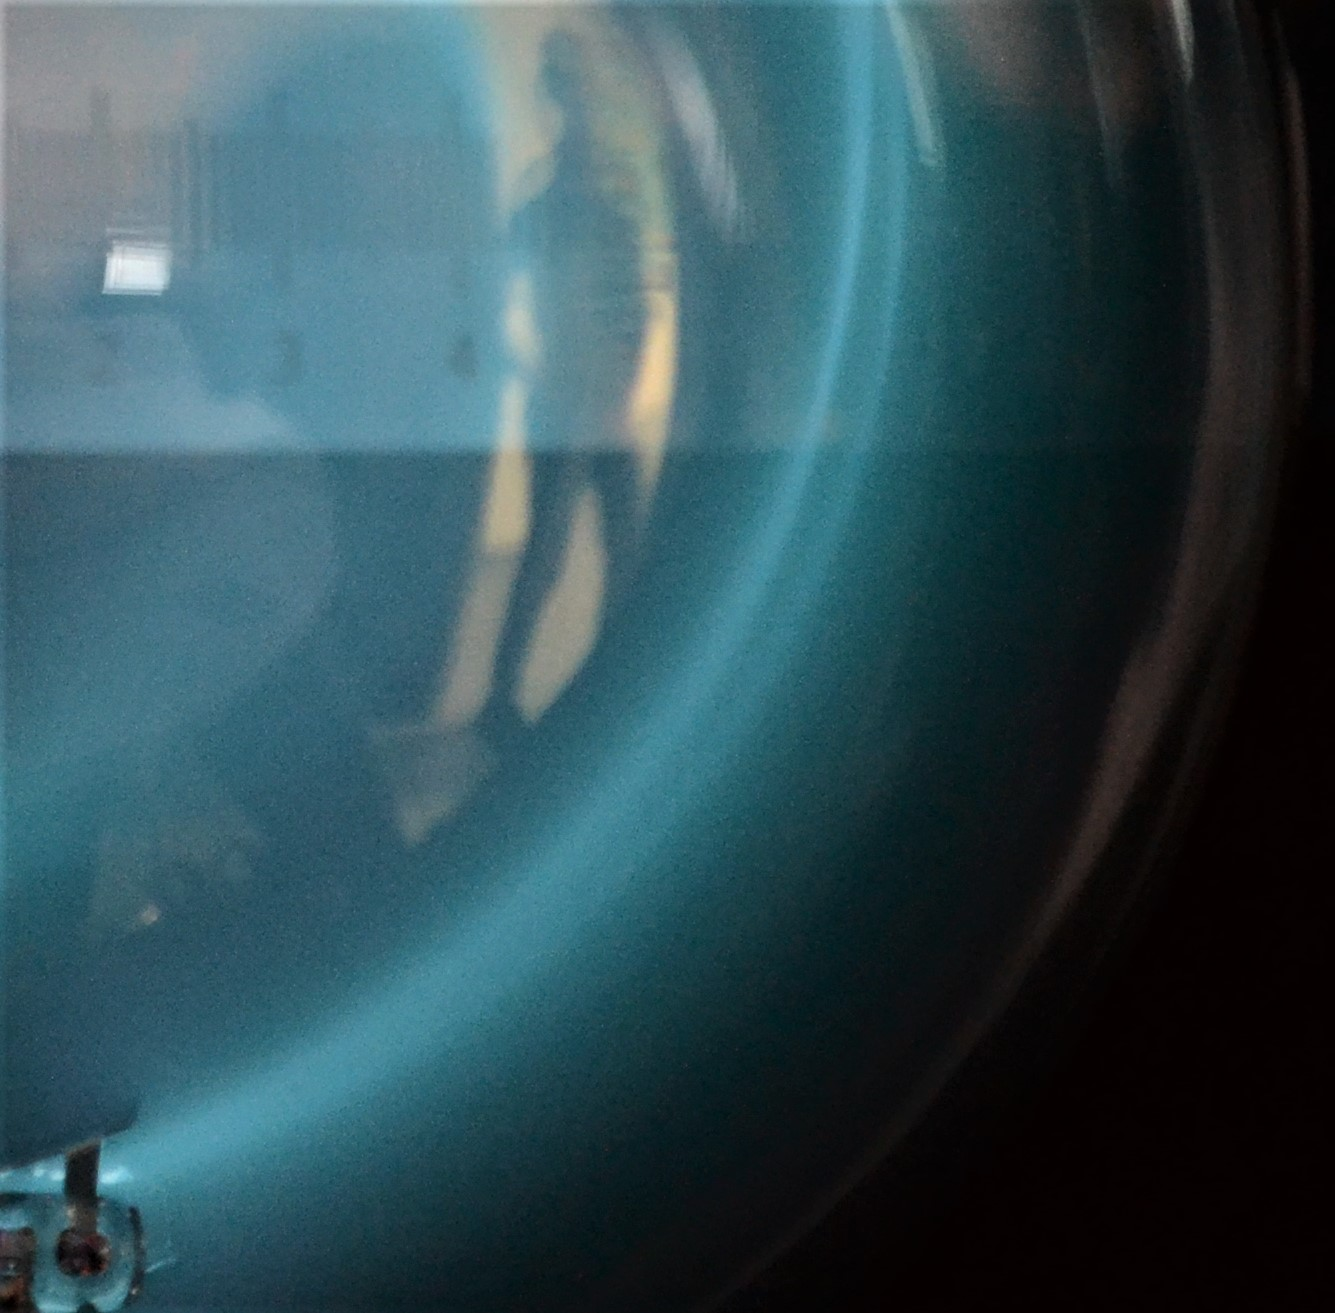
\includegraphics[scale=0.639]{(18).JPG}
			\label{doppio}}
		\subfloat{
			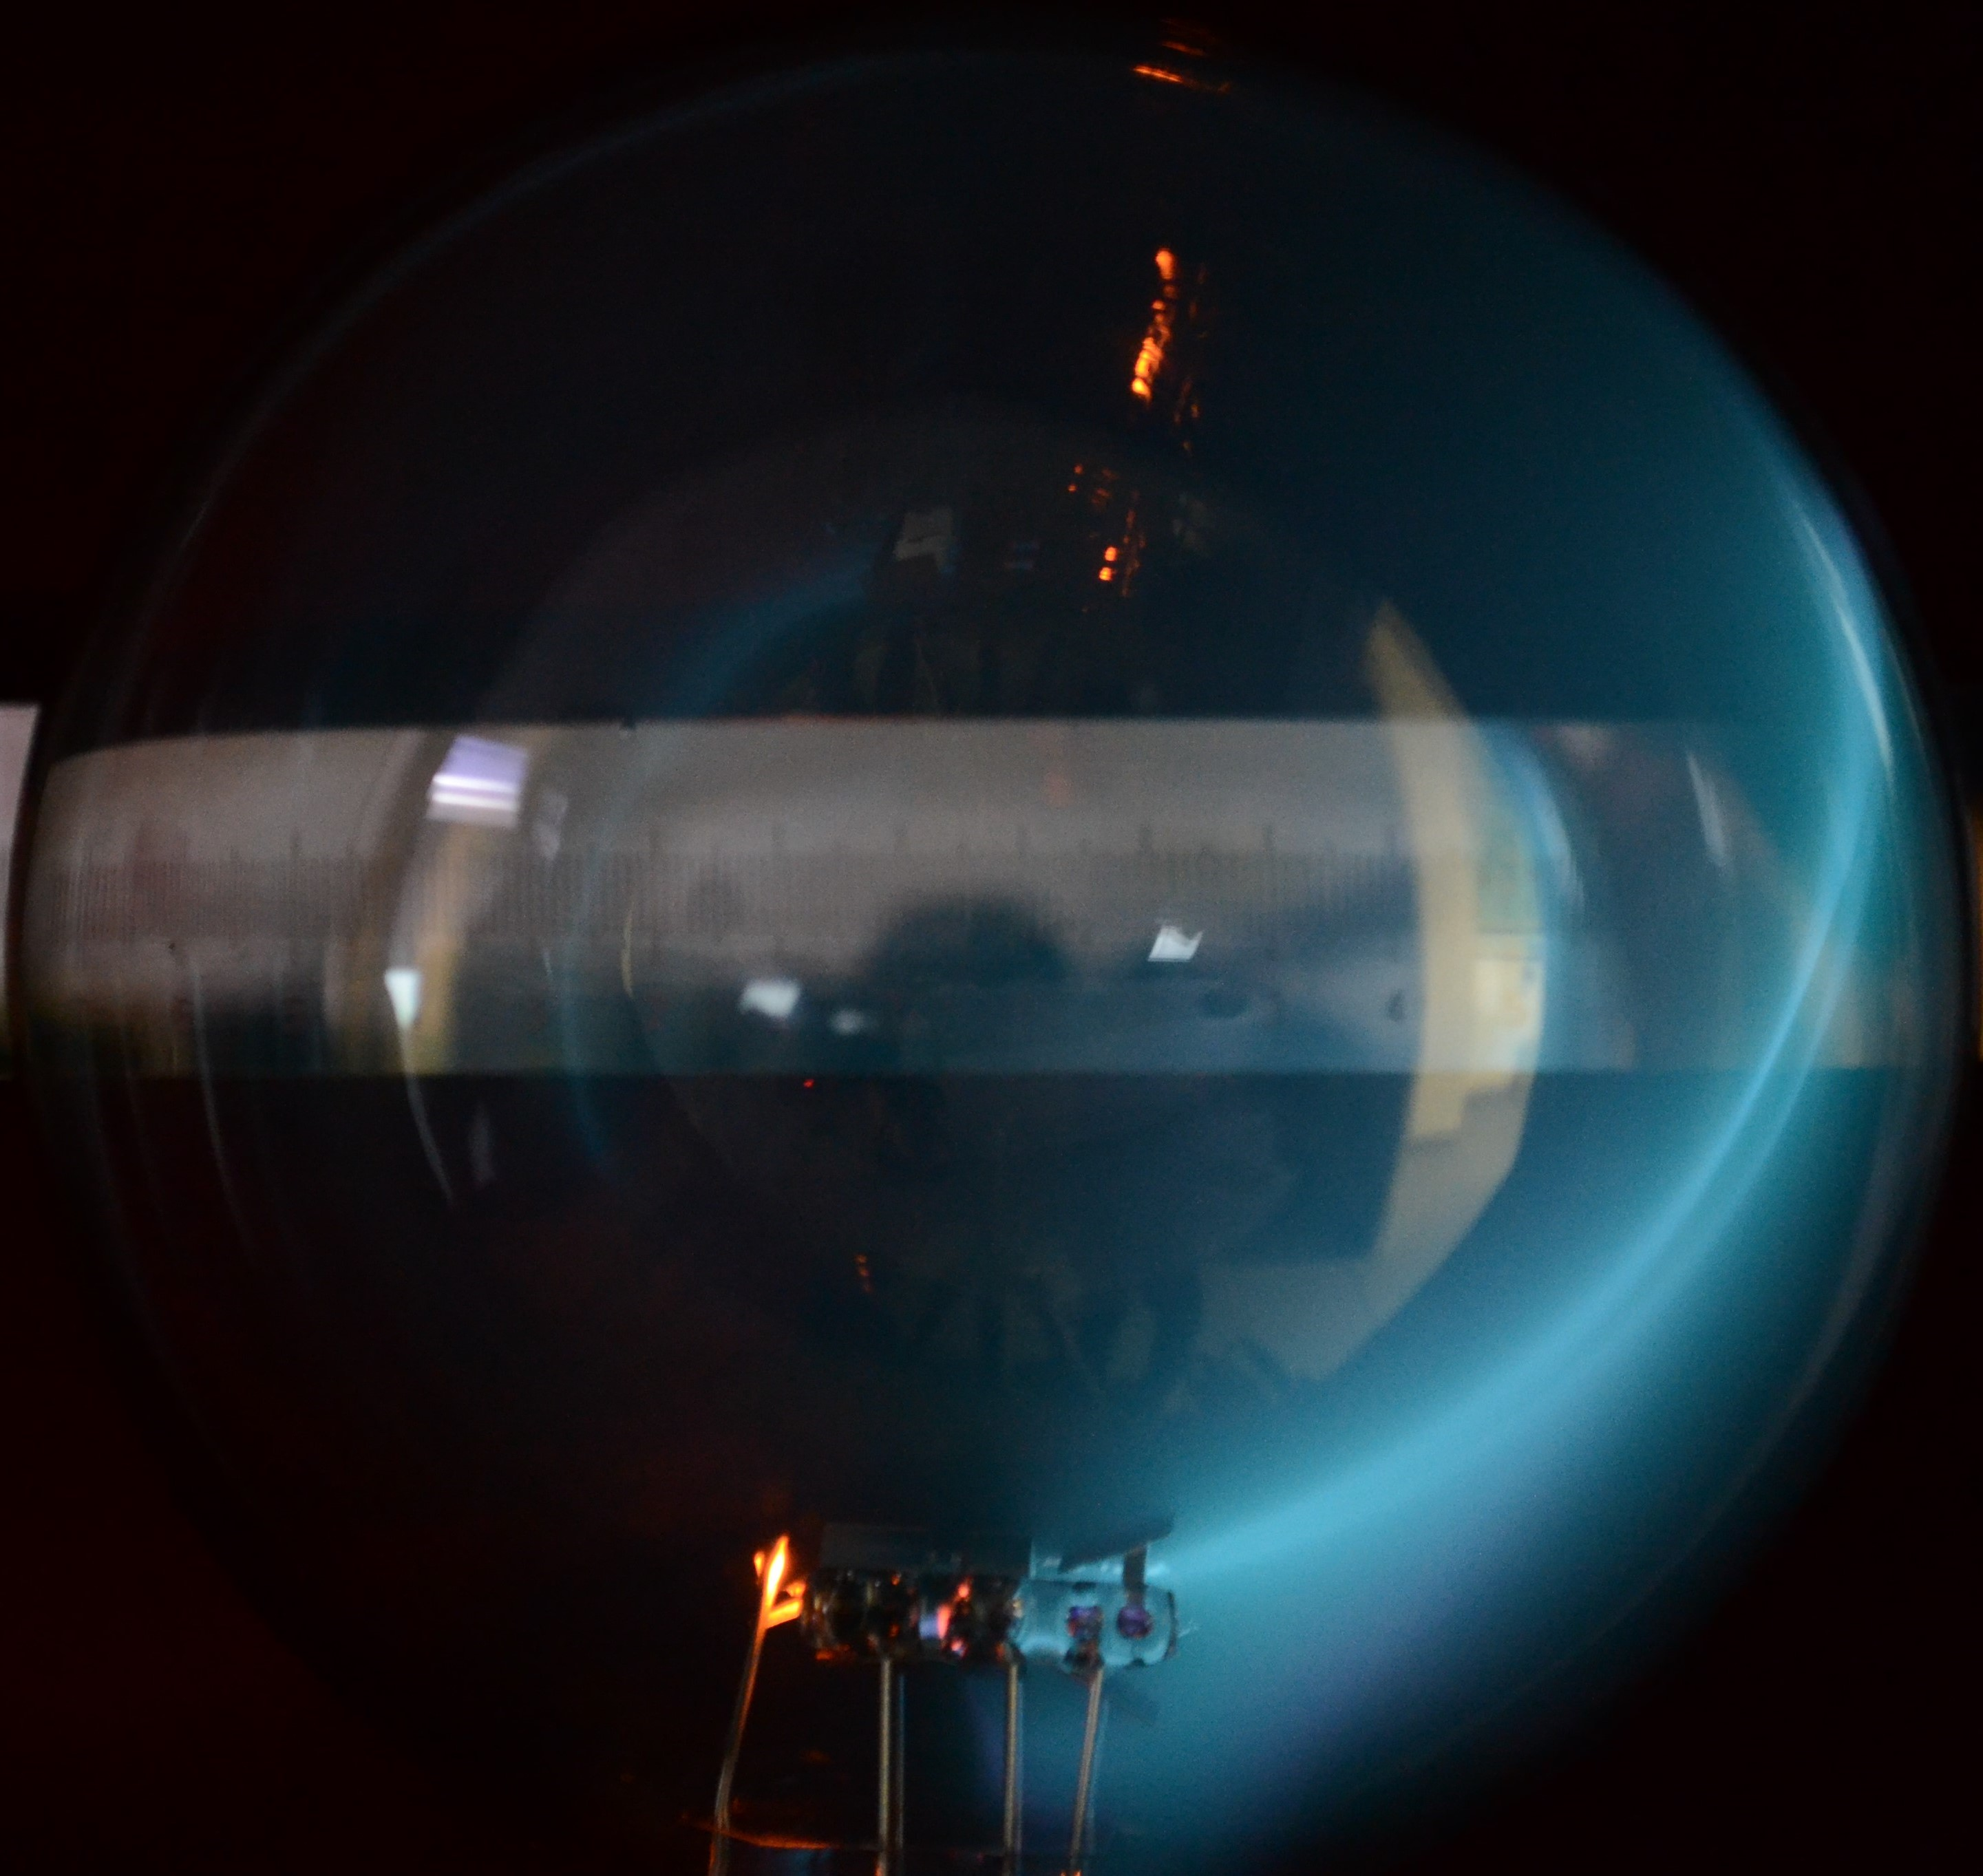
\includegraphics[scale=0.308]{(60).JPG}
			\label{esce}}
		\caption{Esempi di acquisizioni e anomalie}
		\label{f:acquisizione}
	\end{figure}

Dalle foto si possono notare alcuni elementi di cui bisognerà tener conto durante l'analisi:
\begin{itemize}
	\item il fascio, sopratutto per basse tensioni $V$ del cannone elettronico (e conseguentemente basse energie degli elettroni) si affievolisce velocemente per colpa degli urti tra elettroni e atomi di He nel bulbo, questo rende il fascio dai contorni meno netti e aumenta l'incertezza sulla determinazione del raggio;
	\item nelle stesse condizioni del punto precedente il fascio diminuisce evidentemente il raggio di curvatura poiché gli elettroni perdendo energia curvano di più;
	\item il fascio non è ben collimato, in certi punti è visibile come si divida in due parti, aumentando l'incertezza sulla determinazione del raggio;
	\item per alte tensioni $V$ del cannone elettronico ma basse correnti $I$ passanti per le bobine il fascio esce subito dal bulbo, in queste condizioni la porzione di circonferenza visibile è ridotta e si trova tutta sul bordo del bulbo: la parte più soggetta alle distorsioni ottiche dovute allo stesso.
\end{itemize}

Nel seguito si è tenuto conto di questi effetti, ad esempio ignorando la parte finale della traiettoria o scartando le acquisizioni dove è visibile una parte troppo piccola di circonferenza.

In prima battuta fitteremo le circonferenze misurandone il raggio in pixel, quindi valuteremo il fattore di conversione pixel/metri.

\subsection{Fit delle circonferenze} 
Dato l'elevato numero di foto acquisite si è deciso di procedere ad un fit automatico delle circonferenze. Il procedimento seguito si divide in due fasi:
\begin{itemize}
	\item eliminare dalla foto tutti gli elementi estranei alla circonferenza da fittare;
	\item eseguire il fit vero e proprio e valutare l'errore sul raggio.
\end{itemize}

\paragraph{Isolamento delle circonferenze} Si è sfruttato l'alto contrasto delle circonferenze e il loro colore (gli atomi di Elio eccitati emettono per lo più nel blu) per isolarle rispetto agli altri elementi. Utilizzando un software di photo-editing si sono eliminati i canali rosso e verde e tutti i pixel che non avessero luminosità in un certo range (scelto in modo da isolare le sole circonferenze). 

Alla fine di questo procedimento in certe foto è rimasto del segnale riflesso dal righello specchiato che è stato rimosso manualmente.

Un esempio del risultato finale è visibile in \figurename{ \ref{circ}}.

\begin{figure}[H]
	\centering
		\subfloat{
			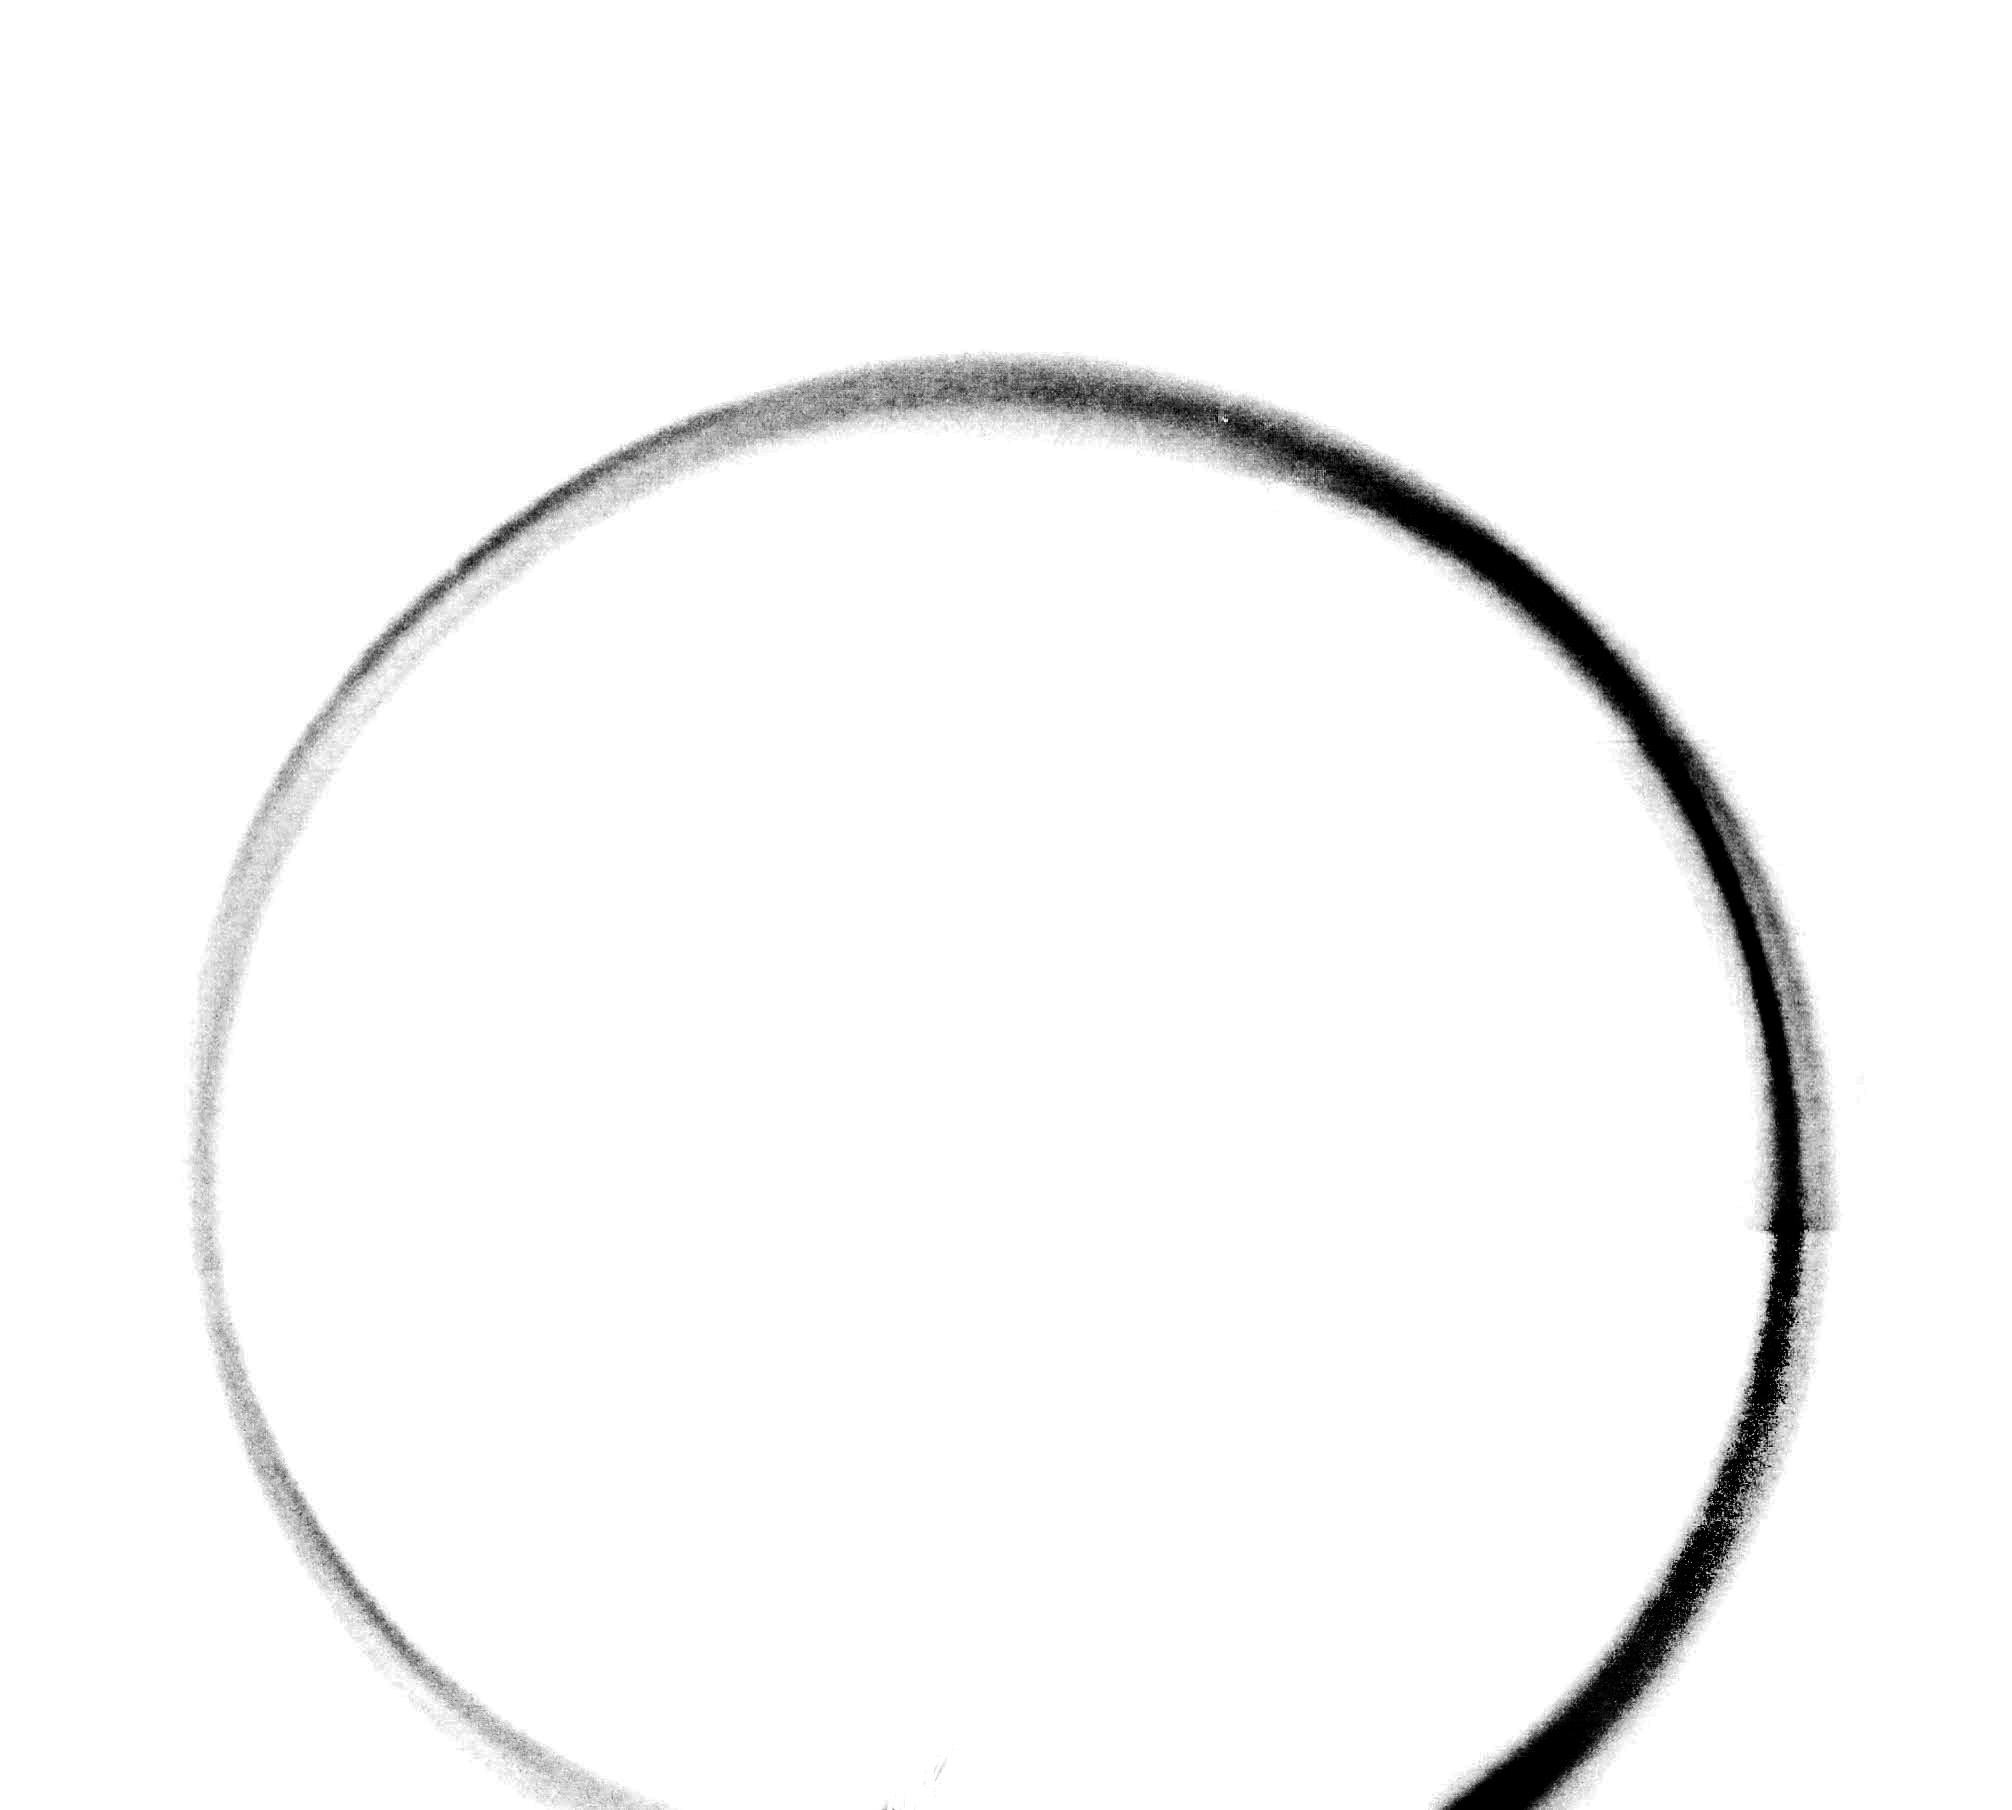
\includegraphics[scale=0.45]{1.JPG}}
		\subfloat{
			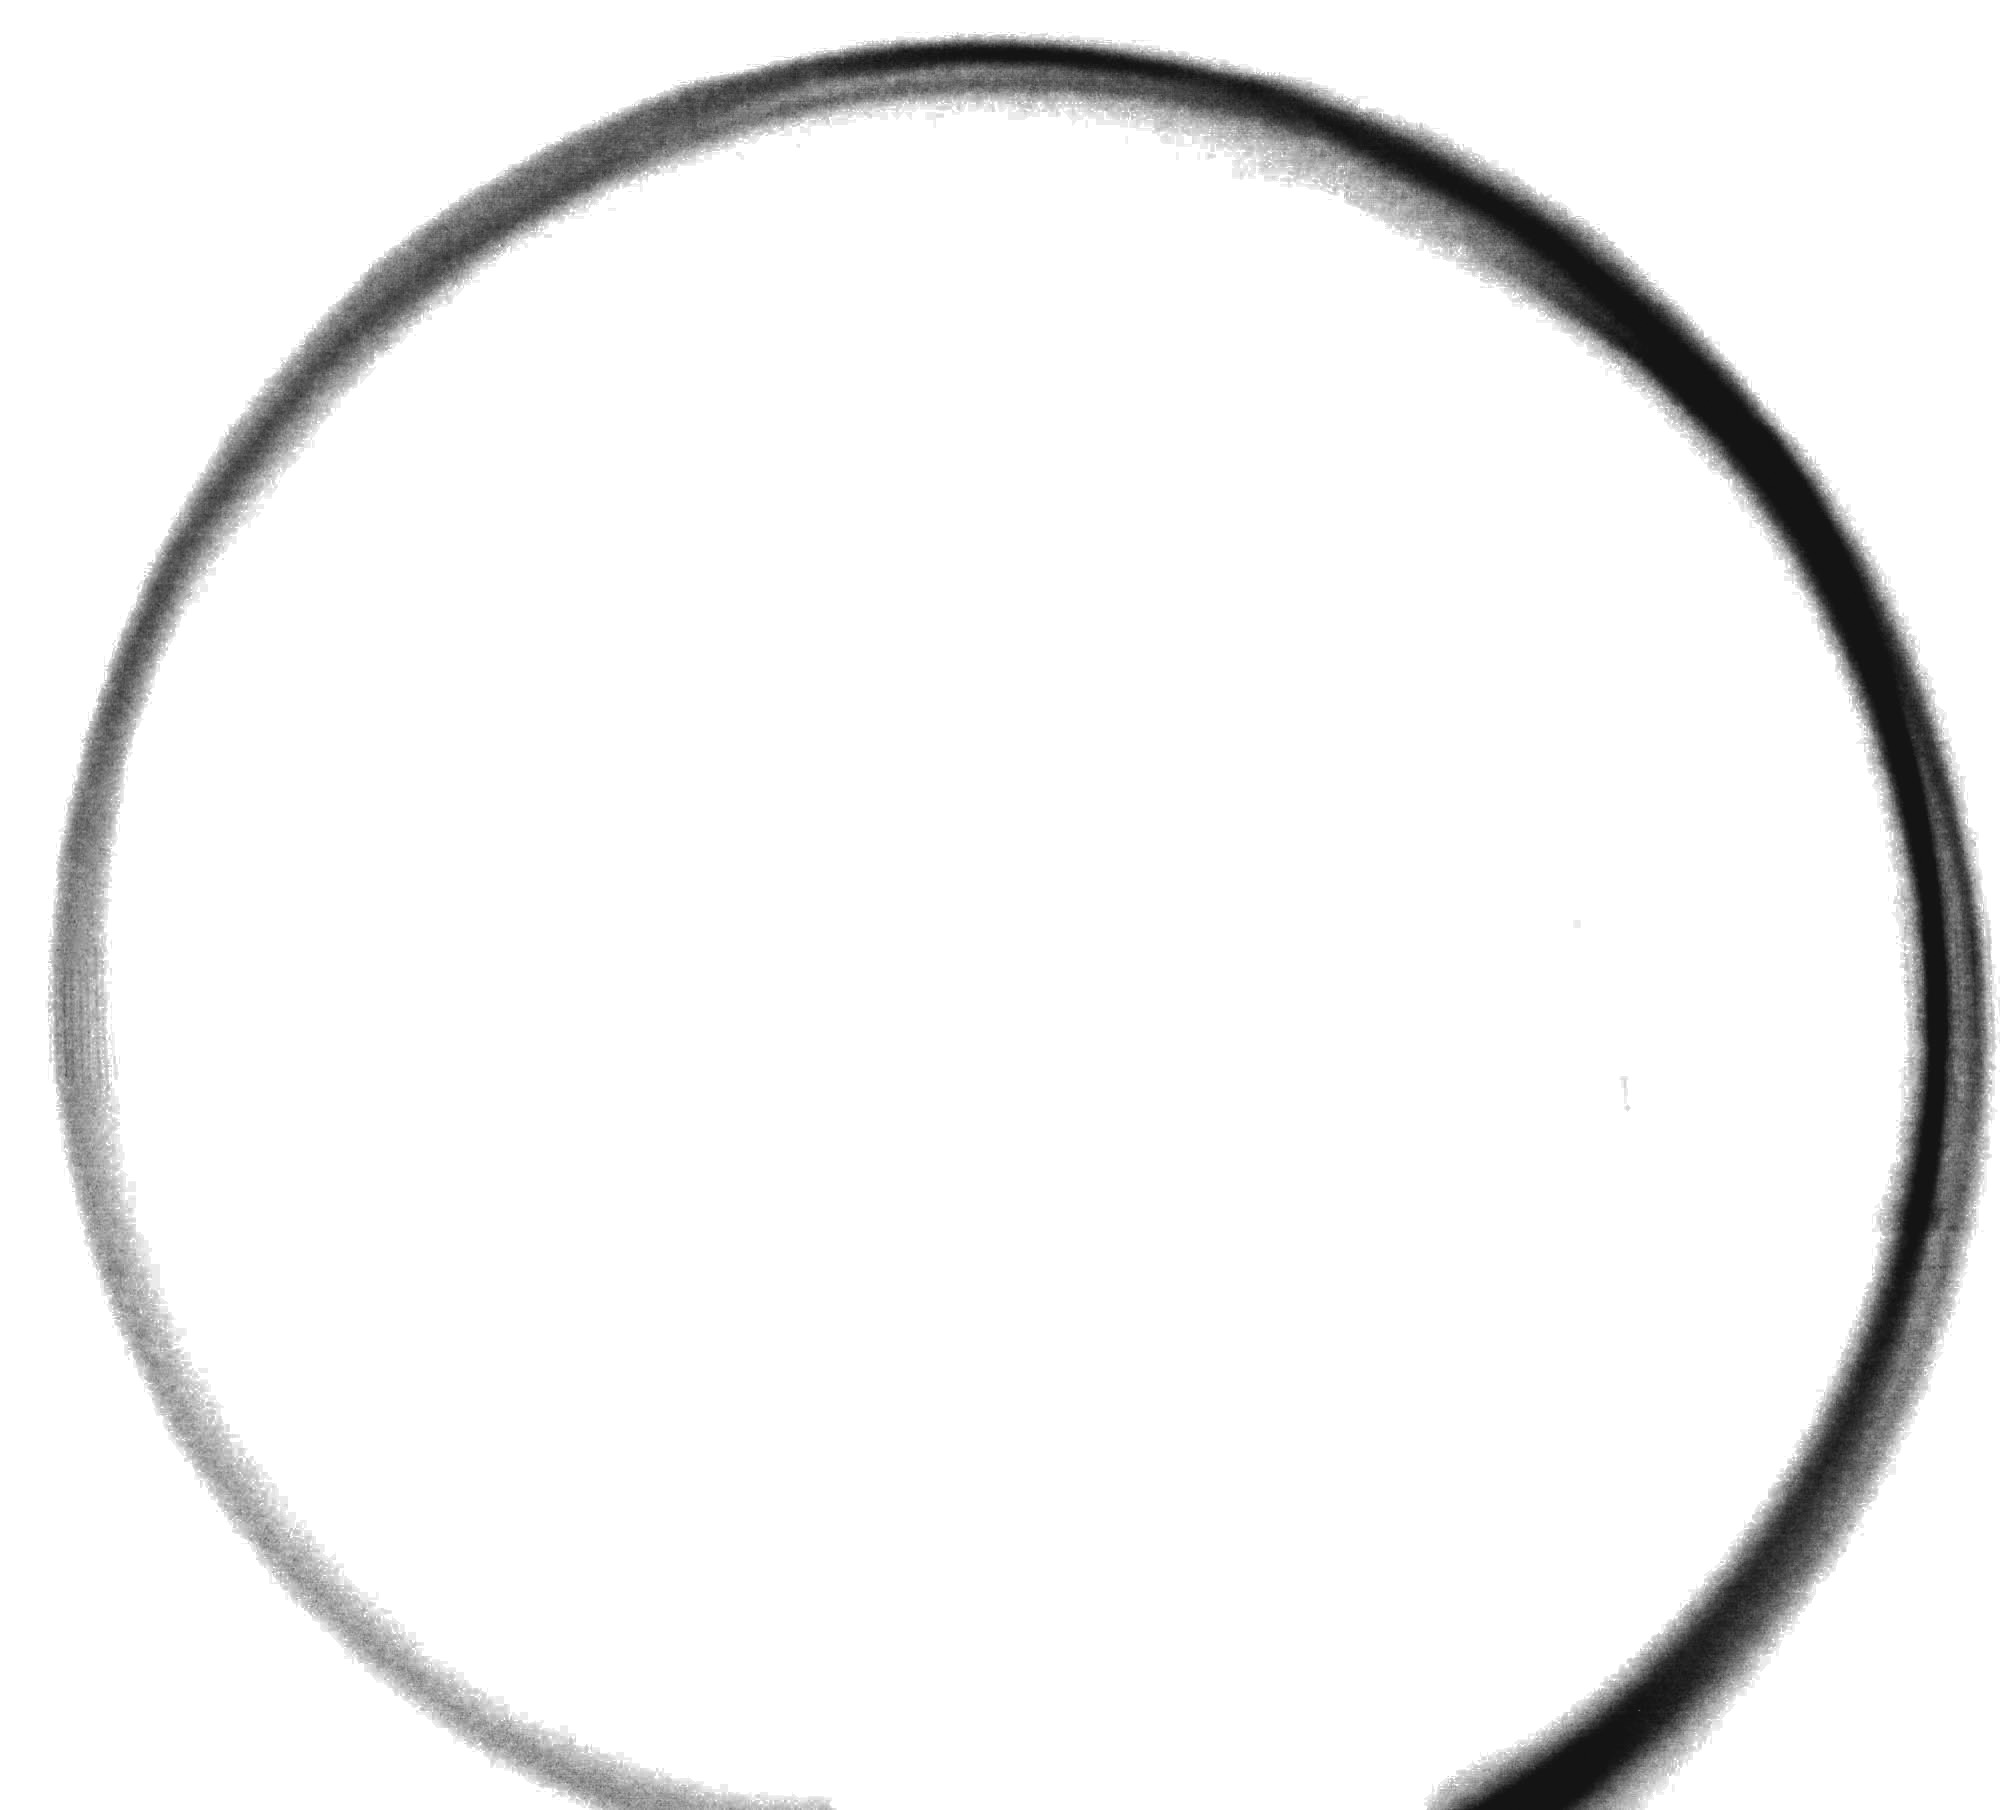
\includegraphics[scale=0.45]{2.JPG}}
	\caption{circonferenze isolate dal background}
	\label{circ}
\end{figure}
%le foto che ho messo non sono nostre, ma di un altro gruppo, ma erano più belline delle nostre quindi...

\paragraph{Fit delle circonferenze} Le circonferenze sono quindi state fittate analiticamente secondo il metodo descritto in \emph{I.Kàsa, "A Circle Fitting Procedure and Its Error Analysis"}: in pratica si è cercata la circonferenza che minimizza la somma delle distanze al quadrato tra la circonferenza stessa e tutti i punti sperimentali.
Nel selezionare i punti sperimentali possiamo decidere di stringere o allargare il range di luminosità entro il quale considerare un punto facente parte della traccia.

Questa soglia è arbitraria (come del resto sarebbe se la scelta dei punti fosse fatta a mano) e si è scelta in modo da eliminare l'ultima parte delle circonferenze: le code come già detto hanno un raggio di curvatura minore avendo gli elettroni perso energia urtando. È visibile, infatti, come al diminuire della soglia di luminosità i raggi fittati diminuiscano leggermente.

\paragraph{Errore sui raggi} Come è chiaro dalle foto delle tracce queste hanno uno spessore non trascurabile, per valutare l'incertezza sulla stima del raggio precedentemente eseguita si è deciso di graficare la distribuzione della lunghezza dei segmenti compresi tra il centro delle circonferenze fittate e i punti sperimentali.
Dopo aver normalizzato la distribuzione per il raggio (altrimenti i punti della traccia più distanti sarebbero più numerosi, essendo la circonferenza più grande) si è deciso di fittarla con una gaussiana di prendere la deviazione standard come errore sulla misura del raggio.

In \figurename{ \ref{gauss}} si riporta, a titolo di esempio, i fit della distribuzione dei raggi di alcune acquisizioni.

\begin{figure}[H]
	\centering
	\subfloat{
		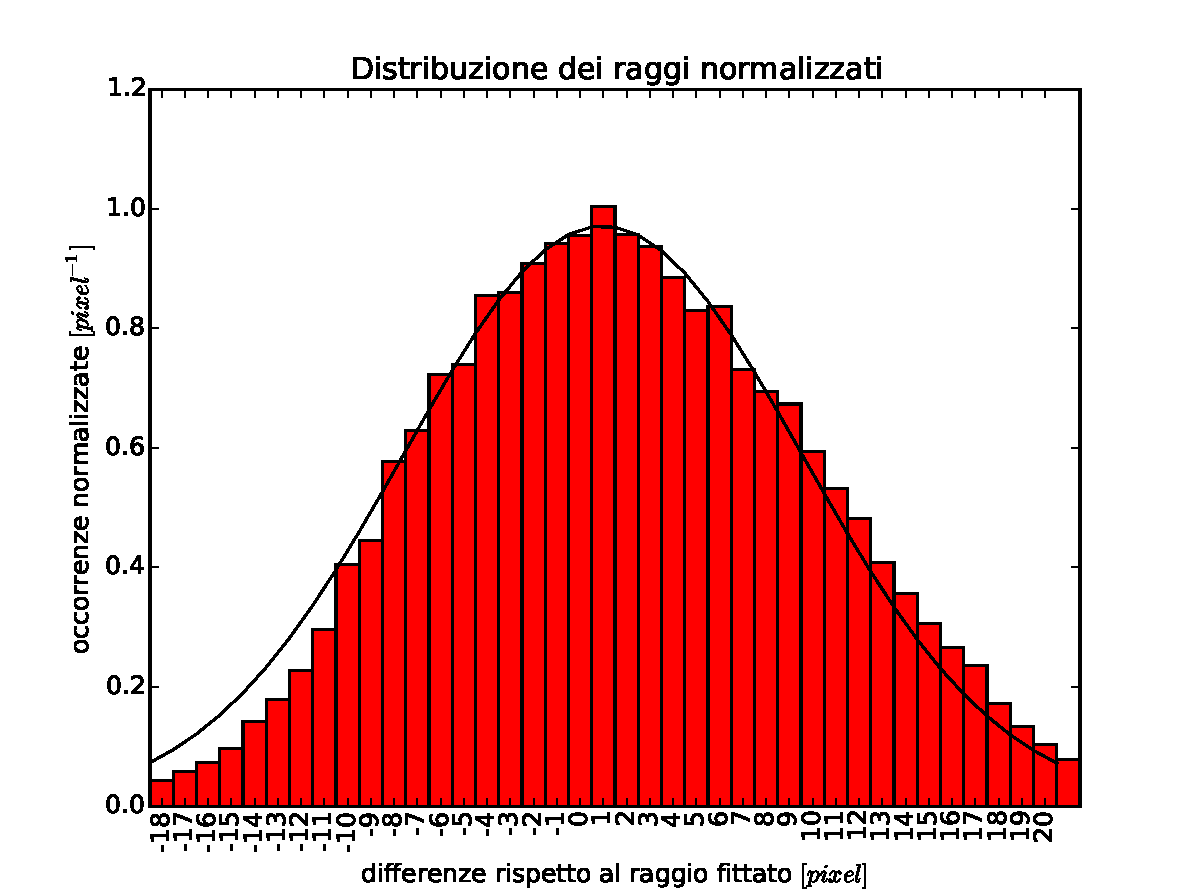
\includegraphics[scale=0.42]{fit_9.pdf}}
	\subfloat{
		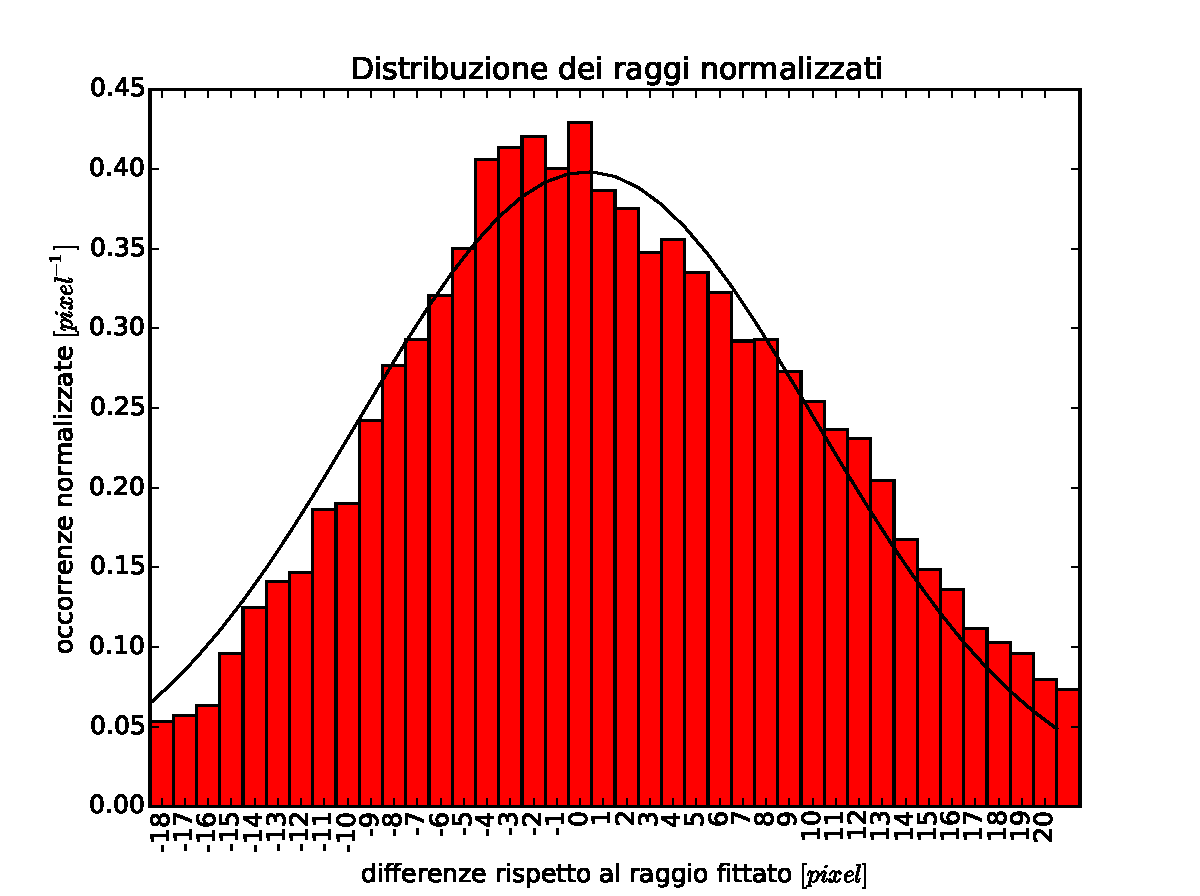
\includegraphics[scale=0.42]{fit_10.pdf}}
	\caption{stima dell'errore sulla misura dei raggi}
	\label{gauss}
\end{figure}

\subsection{Misura del fattore di conversione px/m}

Ottenuta la misura dei raggi e le relative incertezze è necessario convertire la misura da pixel a metri, per farlo si è acquisita una foto del righello nell'apparato, senza il bulbo, come visibile in \figurename{ \ref{righello}}. Si è misurata la distanza tra i due estremi (per minimizzare l'errore sul posizionamento del centro della tacca) e si è preso come errore l'estensione in pixel della tacca sul righello.

Il fattore di conversione così determinato è di $k = \SI{181.9(3)}{px/\cm}$.

Questa prima stima va corretta per per l'effetto della prospettiva (il righello si trova dietro al piano dell'orbita degli elettroni) e per gli effetti di distorsione ottica del bulbo.

\begin{figure}[H]
	\centering
	\includegraphics[scale=0.3]{NO.JPG}
	\caption{foto della scala graduata di calibrazione}
	\label{righello}
\end{figure}

\paragraph{Prospettiva}	Si è misurata la distanza dell'obiettivo della macchina fotografica dal righello e la distanza di questo dal centro del bulbo. Anche se la risoluzione del metro è \SI{1}{\mm} si è valutato di non avere tale precisione nella determinazione del centro del bulbo e nel posizionamento del metro, la misura è stata perciò ripetuta da ogni membro del gruppo e si è preso l'errore massimo. 
% è falso ma è guisto per non dire che il nuovo errore è a caso

I risultati delle misure sono $d_{OR} = \SI{56.5 \pm 0.3}{\cm}$ (distanza obiettivo/righello) e $d_{RB} = \SI{11 \pm 0.2}{\cm}$ (distanza righello/bulbo).
Il fattore di correzione alla misura precedente è di $c = {1.242 \pm 0.003}$, da cui si ottiene una fattore di conversione corretto di $k_c = \SI{225.9 \pm 0.6}{px/\cm}$.

\paragraph{Distorsione del bulbo} Non è banale determinare l'entità della distorsione alla forma delle tracce dovuta alla presenza del bulbo di vetro.

L'osservazione della distorsione prodotta sulla scala graduata del righello non ci da molte informazioni poiché la scala graduata si trova dietro al bulbo e per arrivare all'obiettivo passa due volte per il vetro e l'effetto del primo passaggio è opposto a quello del secondo. La visibile distorsione della scala graduata è dovuta al fatto che dopo il primo passaggio, i raggi proseguono  nel bulbo deviati e urtano la seconda faccia ad un angolo diverso, per cui l'effetto della seconda faccia non è esattamente opposto a quello della prima.

Tuttavia questo effetto è diverso da quello subito dagli oggetti all'interno del bulbo che attraversano una sola faccia e a priori non è detto che abbia lo stesso ordine di grandezza.

Usando l'ottica geometrica una prima approssimazione potrebbe essere quella di considerare localmente il bulbo come un lastra di vetro piatta nel punto di intersezione dei raggi luminosi, come illustrato in \figurename{ \ref{ottica1}}.

\begin{figure}[H]
	\centering
	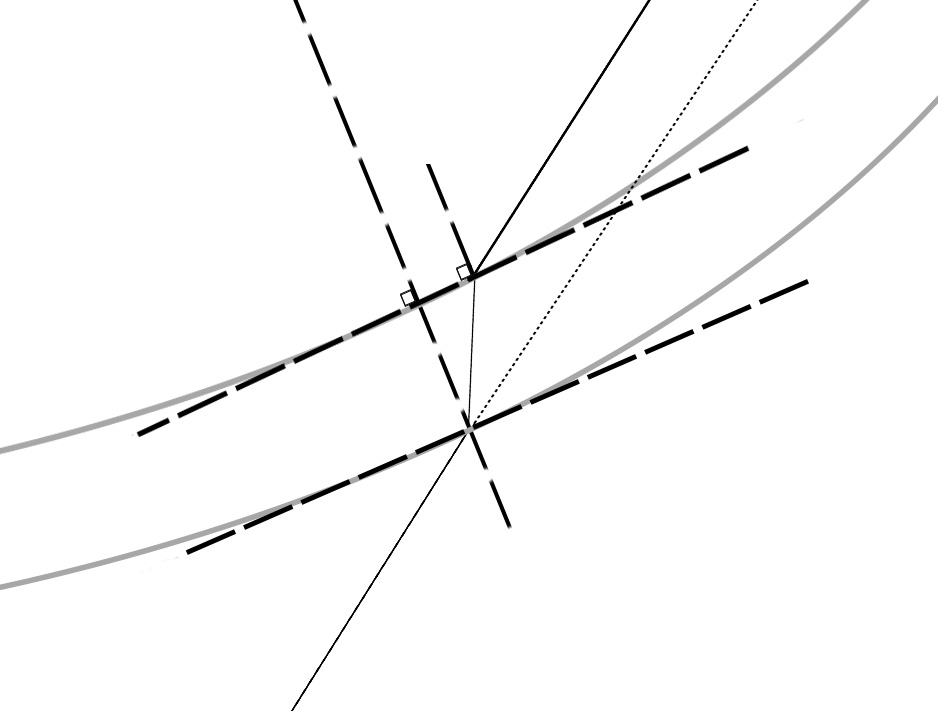
\includegraphics[scale=1]{prima_approx.JPG}
	\caption{schema dei raggi luminosi passanti per il bulbo}
	\label{ottica1}
\end{figure}

I raggi luminosi provenienti dalle tracce (in alto in \figurename{ \ref{ottica1}}) intersecano la superficie interna del bulbo ad una certa inclinazione, proseguono nel vetro con un angolo più piccolo rispetto alla perpendicolare, quindi intersecano la superficie esterna. In questa approssimazione l'angolo di uscita sarà lo stesso di quello di entrata.

Il risultato è che il punto all'interno del bulbo sembrerà più esterno, tuttavia lo spostamento è nel peggiore dei casi pari allo spessore del vetro, che ragionevolmente non sarà più grande di $\SIrange{1}{2}{\mm}$. Rispetto ai raggi tipici misurati ($\sim \SI{5}{\cm}$) si tratterebbe di una correzione dell'ordine del $\sim \SIrange{2}{4}\%$, quindi a priori non trascurabile.

In realtà questa non è una buona approssimazione sul bordo (dove misuriamo buona parte delle nostre tracce), come visibile in \figurename{ \ref{ottica2}}.

\begin{figure}[H]
	\centering
	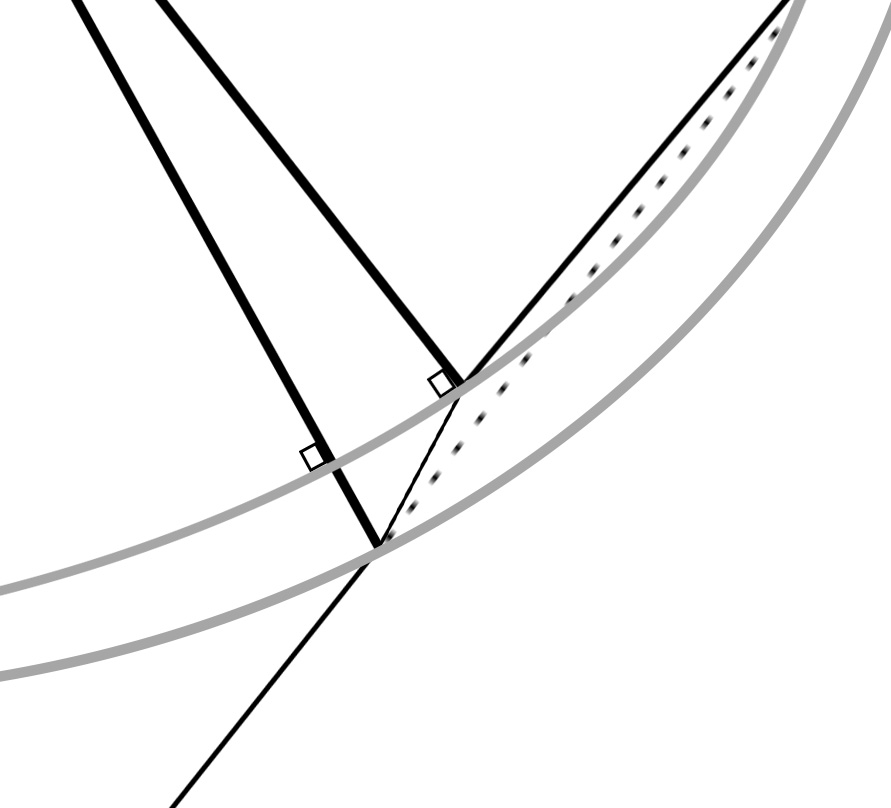
\includegraphics[scale=0.8]{seconda_approx.JPG}
	\caption{schema dei raggi luminosi passanti per il bulbo}
	\label{ottica2}
\end{figure}

Come prima i raggi luminosi provenienti dalle tracce (in alto in \figurename{ \ref{ottica2}}) intersecano la superficie interna ad un certo angolo e proseguono nel vetro come nel caso precedente. Tuttavia la seconda intersezione avviene ad un angolo diverso dal precedente e l'angolo di uscita (rispetto alla perpendicolare) sarà minore.

Il risultato è che in base alla posizione del punto nel bulbo questo potrebbe sembrare più interno. Questo effetto opposto a quello visto sopra potrebbe a priori avere lo stesso ordine di grandezza.

Si è proceduto con l'ottica geometrica al calcolo della funzione che dato il raggio misurato ci dia il raggio corretto e si riporta in \figurename{ \ref{bulbo}} il grafico del fattore di correzione . Nel calcolo si è stimato il raggio del bulbo $R \sim \SI{6.4}{\cm}$ (misurato a partire dalle foto, noto il fattore di conversione prima calcolato), l'indice di rifrazione $n \sim 1.6$ (un vetro generico) e lo spessore di $d \sim \SI{1}{\mm}$.

La correzione finale è quindi dell'ordine del $\SIrange{2}{3}\%$ e solo per raggi maggiori di \SI{6}{\cm}.

\begin{figure}[H]
	\centering
	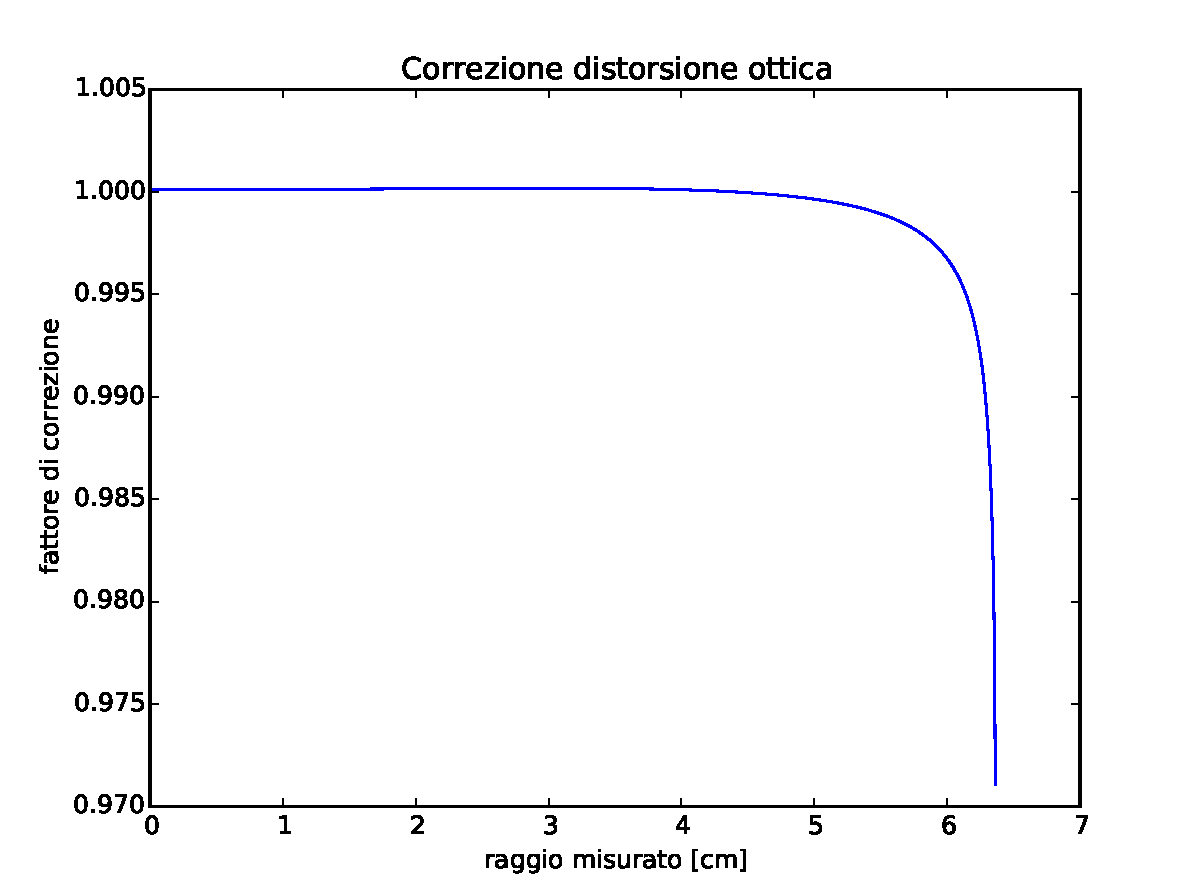
\includegraphics[scale=0.7]{bulbo.pdf}
	\caption{Correzione al fattore di conversione}
	\label{bulbo}
\end{figure}

Nella conversione dei raggi in metri abbiamo tenuto conto di questa correzione facendo quindi l'approssimazione che le circonferenze abbiano centro nel centro del bulbo.
I dati relativi a tutte le acquisizione effettuate, i raggi fittati e i relativi errori sono riportati in appendice in \tablename{ \ref{dati_raggi}}.

\section{Misura di $V$}
La misura di $V$ è fatta dal generatore di tensione del cannone elettronico ed è nota con una risoluzione di \SI{1}{\volt} che si è assunto come errore (andrebbe aggiunto l'errore di calibrazione che è ignoto).

La misura di $V$ è correlata alla determinazione della velocità degli elettroni in uscita dal cannone elettronico e come fatto notare nel datasheet dell'apparato la più grande sorgente di errore nell'esperimento è la non uniformità del campo accelerante, causato dal buco nell'anodo che porta la velocità degli elettroni ad essere inferiore a quella attesa, per cui la misura di $\tfrac{e}{m}$ sarà fortemente affetta da questo effetto.

Non è possibile tenere conto di questi effetti a meno di conoscere esattamente la geometria del cannone elettronico, sappiamo comunque che l'effetto sarà quello di aumentare il valore di  $\tfrac{e}{m}$ sperimentale rispetto a quello teorico.

\section{Calcolo di e/m}
A partire dalle misure effettuate si è proceduto al calcolo di $\tfrac{e}{m}$, si sono quindi mediate le misure a pari $V$ e, tenuto conto di tutte le correzioni esposte nei punti precedenti, i risultati sono i seguenti:

\begin{table}[H]
	\centering
	\begin{tabular}{ccc}
		\toprule
		$V$ [\si{\volt}] & 	$\frac{e}{m} \times 10^{11}$ [C/Kg] \\
		\midrule
$	200 \pm 1	$ & $	2.76 \pm 0.08	$ \\
$	219 \pm 1	$ & $	2.81 \pm 0.08	$ \\
$	232 \pm 1	$ & $	2.83 \pm 0.09	$ \\
$	261 \pm 1	$ & $	2.92 \pm 0.10	$ \\
$	282 \pm 1	$ & $	2.97 \pm 0.10	$ \\
$	302 \pm 1	$ & $	2.97 \pm 0.13	$ \\
\bottomrule
\end{tabular}
\end{table}

\section{Conclusioni}
Come è chiaro i risultati sono assolutamente incompatibili con il valore noto di $\SI{1.76e11}{C/Kg}$.

Tuttavia questo risultato era atteso: il datasheet dell'apparato riporta che con questa strumentazione, dato l'errore sulla velocità, il risultato della misura di $\tfrac{e}{m}$ eccederà il valore noto di $\sim \SI{1.1e11}{C/Kg}$.
È possibile confrontare il grafico presente nel datasheet riportato in \figurename{ \ref{grafico_farlocco}} con i risulti delle nostre misure in \figurename{ \ref{dati_nostri}} e notare che i valori trovati sono compatibili.

\begin{figure}[H]
	\centering
		\begin{minipage}{0.5\textwidth}
			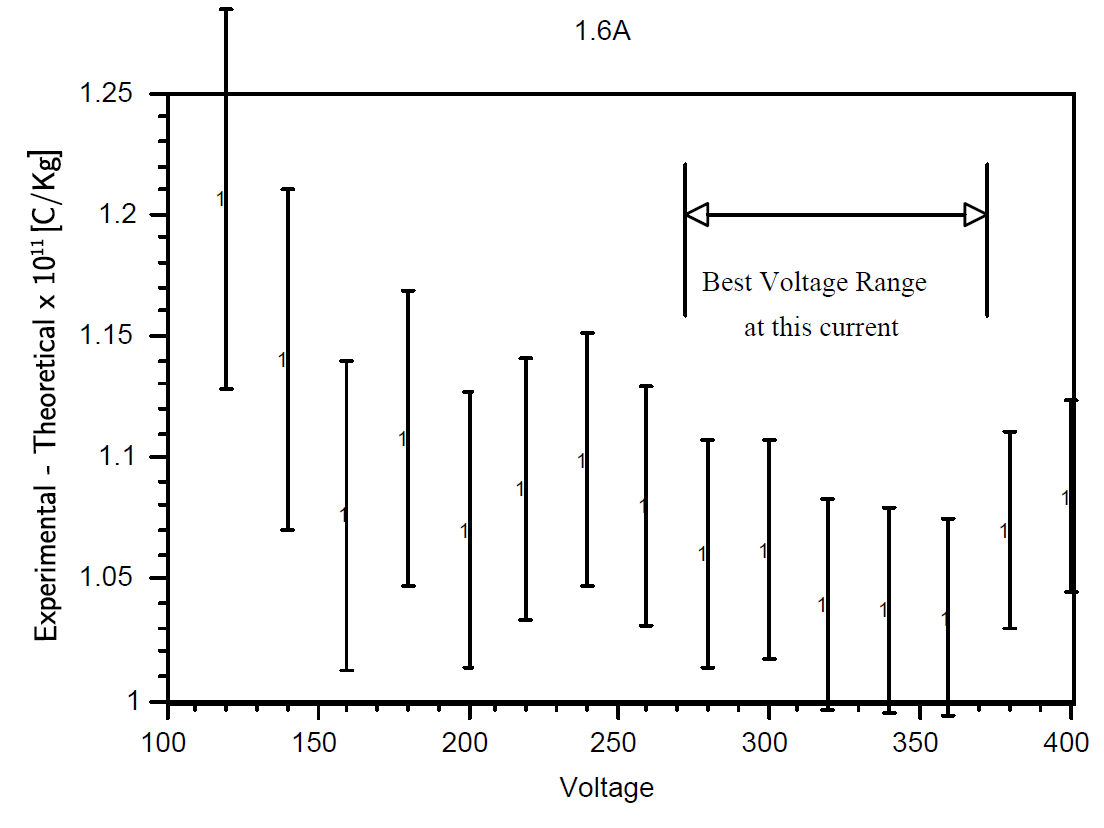
\includegraphics[scale=0.22]{farlocco.png}
			\caption{datasheet dell'apparato}
			\label{grafico_farlocco}
		\end{minipage}
		\begin{minipage}{0.49\textwidth}
			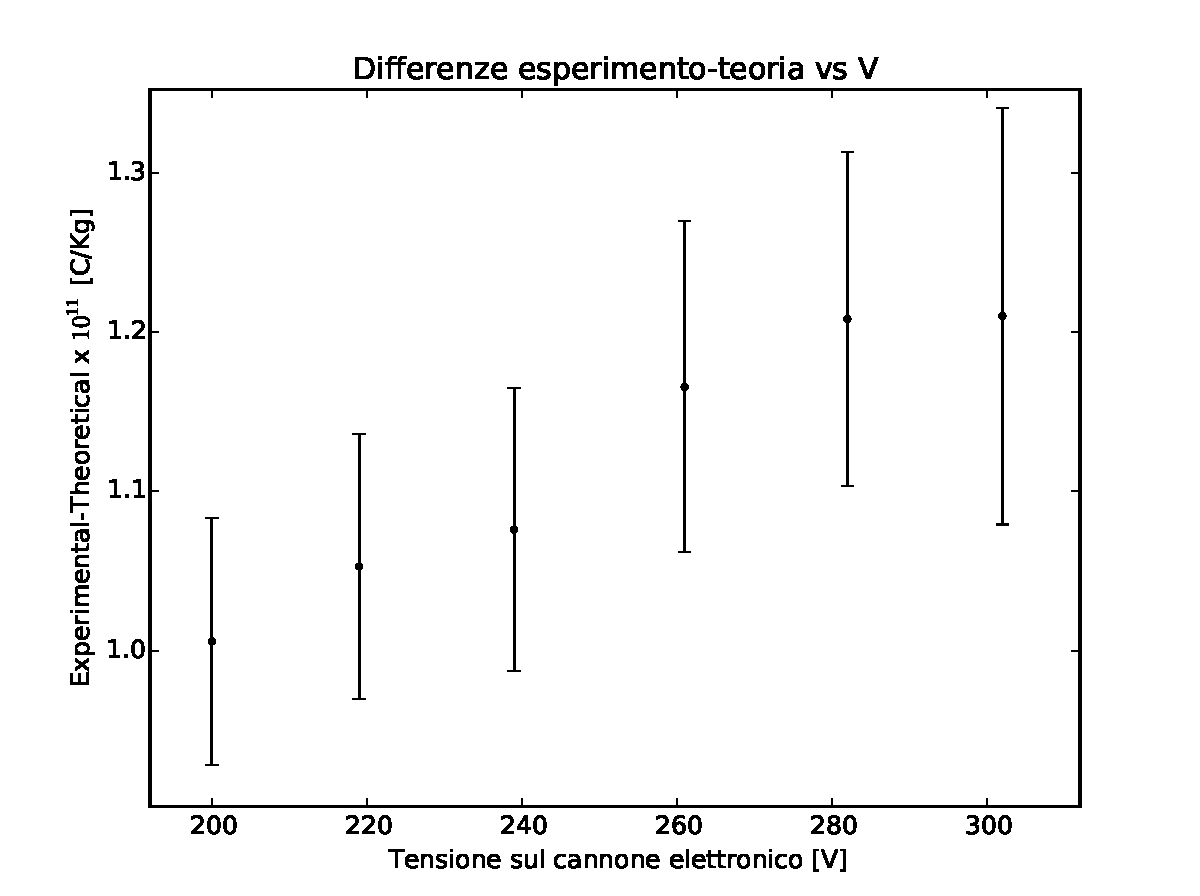
\includegraphics[scale=0.45]{dm.pdf}
			\caption{misure ottenute}
			\label{dati_nostri}
		\end{minipage}
\end{figure}

\newpage
\section{Appendice}
\begin{figure}[h!]
\begin{minipage}{0.49\textwidth}
		\centering
		\begin{tabular}{ccccc}
			\toprule
			$l$ [\si{cm}]	& 	$V_{out}$ [\si{\volt}]	&& 	$l$ [\si{cm}]	& 	$V_{out}$ [\si{\volt}] \\
			\midrule
			14.0 	& 	 0.405	&&	25.5	& 	 0.407 \\
			14.5	& 	 0.407	&&	20.5	& 	 0.410 \\
			15.0	& 	 0.408	&&	21.0	& 	 0.410 \\
			15.5	& 	 0.408	&&	21.5	& 	 0.409 \\
			16.0	& 	 0.408	&&	22.0	& 	 0.410 \\
			16.5	& 	 0.409	&&	22.5	& 	 0.410 \\
			17.0	& 	 0.409	&&	23.0	& 	 0.410 \\
			17.5	& 	 0.409	&&	23.5	& 	 0.409 \\
			18.0	& 	 0.409	&&	24.0	& 	 0.409 \\
			18.5	& 	 0.409	&&	24.5	& 	 0.409 \\
			19.0	& 	 0.409	&&	25.0	& 	 0.408 \\
			19.5	& 	 0.409	&&	25.0	& 	 0.408 \\
			20.0	& 	 0.409	&&	26.0	& 	 0.406 \\
			\bottomrule
		\end{tabular}
		\captionof{table}{Mappatura del campo magnetico all'interno della bobina di Helmholtz.}
		\label{tab:a}
\end{minipage}
\begin{minipage}{0.49\textwidth}
	\centering
\begin{tabular}{ccc}
	\toprule
$V$ [\si{\volt}] & 	$I$ [\si{\ampere}] & $r$ [\si{\cm}]\\
\midrule
$200	\pm 1 $	 	&	$0.99 \pm 0.01 $	&	$1104 \pm 	11$	\\
$200	\pm 1 $		&	$1.03 \pm 0.01 $	&	$1077 \pm 	10$	\\
$200	\pm 1 $		&	$1.07 \pm 0.01 $	&	$1041 \pm 	9$	\\
$200	\pm 1 $		&	$1.10 \pm 0.01 $	&	$1015 \pm 	10$	\\
$200	\pm 1 $		&	$1.15 \pm 0.01 $	&	$935 \pm  	11$	\\
$219	\pm 1 $		&	$1.03 \pm 0.01 $	&	$1108 \pm 	16$	\\
$219	\pm 1 $		&	$1.07 \pm 0.01 $	&	$1097 \pm 	13$	\\
$219	\pm 1 $		&	$1.10 \pm 0.01 $	&	$1056 \pm 	16$	\\
$219	\pm 1 $		&	$1.15 \pm 0.01 $	&	$1044 \pm 	16$	\\
$239	\pm 1 $		&	$1.07 \pm 0.01 $	&	$1099 \pm 	18$	\\
$239	\pm 1 $		&	$1.15 \pm 0.01 $	&	$1075 \pm 	17$	\\
$261	\pm 1 $		&	$1.07 \pm 0.01 $	&	$1110 \pm 	18$	\\
$261	\pm 1 $		&	$1.10 \pm 0.01 $	&	$1109 \pm 	17$	\\
$261	\pm 1 $		&	$1.14 \pm 0.01 $	&	$1091 \pm 	16$	\\
$282	\pm 1 $		&	$1.07 \pm 0.01 $	&	$1199 \pm 	16$	\\
$282	\pm 1 $		&	$1.10 \pm 0.01 $	&	$1124 \pm 	20$	\\
$282	\pm 1 $		&	$1.15 \pm 0.01 $	&	$1106 \pm 	20$	\\
$302	\pm 1 $		&	$1.10 \pm 0.01 $	&	$1193 \pm 	19$	\\
$302	\pm 1 $		&	$1.15 \pm 0.01 $	&	$1123 \pm 	21$	\\
\bottomrule
\end{tabular}
\captionof{table}{Dati di tutte le acquisizioni}
\label{dati_raggi}
\end{minipage}

\end{figure}

	
	
	
	
	
	
	
	
	
	
	
	
	
	
	
	
	
	
	
	
	
	